\documentclass[]{article}
\usepackage{lmodern}
\usepackage{amssymb,amsmath}
\usepackage{ifxetex,ifluatex}
\usepackage{fixltx2e} % provides \textsubscript
\ifnum 0\ifxetex 1\fi\ifluatex 1\fi=0 % if pdftex
  \usepackage[T1]{fontenc}
  \usepackage[utf8]{inputenc}
\else % if luatex or xelatex
  \ifxetex
    \usepackage{mathspec}
  \else
    \usepackage{fontspec}
  \fi
  \defaultfontfeatures{Ligatures=TeX,Scale=MatchLowercase}
\fi
% use upquote if available, for straight quotes in verbatim environments
\IfFileExists{upquote.sty}{\usepackage{upquote}}{}
% use microtype if available
\IfFileExists{microtype.sty}{%
\usepackage{microtype}
\UseMicrotypeSet[protrusion]{basicmath} % disable protrusion for tt fonts
}{}
\usepackage[margin=1in]{geometry}
\usepackage{hyperref}
\hypersetup{unicode=true,
            pdftitle={Aquaculture Model - Demo},
            pdfborder={0 0 0},
            breaklinks=true}
\urlstyle{same}  % don't use monospace font for urls
\usepackage{color}
\usepackage{fancyvrb}
\newcommand{\VerbBar}{|}
\newcommand{\VERB}{\Verb[commandchars=\\\{\}]}
\DefineVerbatimEnvironment{Highlighting}{Verbatim}{commandchars=\\\{\}}
% Add ',fontsize=\small' for more characters per line
\usepackage{framed}
\definecolor{shadecolor}{RGB}{248,248,248}
\newenvironment{Shaded}{\begin{snugshade}}{\end{snugshade}}
\newcommand{\KeywordTok}[1]{\textcolor[rgb]{0.13,0.29,0.53}{\textbf{#1}}}
\newcommand{\DataTypeTok}[1]{\textcolor[rgb]{0.13,0.29,0.53}{#1}}
\newcommand{\DecValTok}[1]{\textcolor[rgb]{0.00,0.00,0.81}{#1}}
\newcommand{\BaseNTok}[1]{\textcolor[rgb]{0.00,0.00,0.81}{#1}}
\newcommand{\FloatTok}[1]{\textcolor[rgb]{0.00,0.00,0.81}{#1}}
\newcommand{\ConstantTok}[1]{\textcolor[rgb]{0.00,0.00,0.00}{#1}}
\newcommand{\CharTok}[1]{\textcolor[rgb]{0.31,0.60,0.02}{#1}}
\newcommand{\SpecialCharTok}[1]{\textcolor[rgb]{0.00,0.00,0.00}{#1}}
\newcommand{\StringTok}[1]{\textcolor[rgb]{0.31,0.60,0.02}{#1}}
\newcommand{\VerbatimStringTok}[1]{\textcolor[rgb]{0.31,0.60,0.02}{#1}}
\newcommand{\SpecialStringTok}[1]{\textcolor[rgb]{0.31,0.60,0.02}{#1}}
\newcommand{\ImportTok}[1]{#1}
\newcommand{\CommentTok}[1]{\textcolor[rgb]{0.56,0.35,0.01}{\textit{#1}}}
\newcommand{\DocumentationTok}[1]{\textcolor[rgb]{0.56,0.35,0.01}{\textbf{\textit{#1}}}}
\newcommand{\AnnotationTok}[1]{\textcolor[rgb]{0.56,0.35,0.01}{\textbf{\textit{#1}}}}
\newcommand{\CommentVarTok}[1]{\textcolor[rgb]{0.56,0.35,0.01}{\textbf{\textit{#1}}}}
\newcommand{\OtherTok}[1]{\textcolor[rgb]{0.56,0.35,0.01}{#1}}
\newcommand{\FunctionTok}[1]{\textcolor[rgb]{0.00,0.00,0.00}{#1}}
\newcommand{\VariableTok}[1]{\textcolor[rgb]{0.00,0.00,0.00}{#1}}
\newcommand{\ControlFlowTok}[1]{\textcolor[rgb]{0.13,0.29,0.53}{\textbf{#1}}}
\newcommand{\OperatorTok}[1]{\textcolor[rgb]{0.81,0.36,0.00}{\textbf{#1}}}
\newcommand{\BuiltInTok}[1]{#1}
\newcommand{\ExtensionTok}[1]{#1}
\newcommand{\PreprocessorTok}[1]{\textcolor[rgb]{0.56,0.35,0.01}{\textit{#1}}}
\newcommand{\AttributeTok}[1]{\textcolor[rgb]{0.77,0.63,0.00}{#1}}
\newcommand{\RegionMarkerTok}[1]{#1}
\newcommand{\InformationTok}[1]{\textcolor[rgb]{0.56,0.35,0.01}{\textbf{\textit{#1}}}}
\newcommand{\WarningTok}[1]{\textcolor[rgb]{0.56,0.35,0.01}{\textbf{\textit{#1}}}}
\newcommand{\AlertTok}[1]{\textcolor[rgb]{0.94,0.16,0.16}{#1}}
\newcommand{\ErrorTok}[1]{\textcolor[rgb]{0.64,0.00,0.00}{\textbf{#1}}}
\newcommand{\NormalTok}[1]{#1}
\usepackage{longtable,booktabs}
\usepackage{graphicx,grffile}
\makeatletter
\def\maxwidth{\ifdim\Gin@nat@width>\linewidth\linewidth\else\Gin@nat@width\fi}
\def\maxheight{\ifdim\Gin@nat@height>\textheight\textheight\else\Gin@nat@height\fi}
\makeatother
% Scale images if necessary, so that they will not overflow the page
% margins by default, and it is still possible to overwrite the defaults
% using explicit options in \includegraphics[width, height, ...]{}
\setkeys{Gin}{width=\maxwidth,height=\maxheight,keepaspectratio}
\IfFileExists{parskip.sty}{%
\usepackage{parskip}
}{% else
\setlength{\parindent}{0pt}
\setlength{\parskip}{6pt plus 2pt minus 1pt}
}
\setlength{\emergencystretch}{3em}  % prevent overfull lines
\providecommand{\tightlist}{%
  \setlength{\itemsep}{0pt}\setlength{\parskip}{0pt}}
\setcounter{secnumdepth}{0}
% Redefines (sub)paragraphs to behave more like sections
\ifx\paragraph\undefined\else
\let\oldparagraph\paragraph
\renewcommand{\paragraph}[1]{\oldparagraph{#1}\mbox{}}
\fi
\ifx\subparagraph\undefined\else
\let\oldsubparagraph\subparagraph
\renewcommand{\subparagraph}[1]{\oldsubparagraph{#1}\mbox{}}
\fi

%%% Use protect on footnotes to avoid problems with footnotes in titles
\let\rmarkdownfootnote\footnote%
\def\footnote{\protect\rmarkdownfootnote}

%%% Change title format to be more compact
\usepackage{titling}

% Create subtitle command for use in maketitle
\newcommand{\subtitle}[1]{
  \posttitle{
    \begin{center}\large#1\end{center}
    }
}

\setlength{\droptitle}{-2em}

  \title{Aquaculture Model - Demo}
    \pretitle{\vspace{\droptitle}\centering\huge}
  \posttitle{\par}
    \author{}
    \preauthor{}\postauthor{}
      \predate{\centering\large\emph}
  \postdate{\par}
    \date{2018-12-02}

\usepackage{booktabs}
\usepackage{longtable}
\usepackage{array}
\usepackage{multirow}
\usepackage[table]{xcolor}
\usepackage{wrapfig}
\usepackage{float}
\usepackage{colortbl}
\usepackage{pdflscape}
\usepackage{tabu}
\usepackage{threeparttable}
\usepackage{threeparttablex}
\usepackage[normalem]{ulem}
\usepackage{makecell}

\begin{document}
\maketitle

\subparagraph{Objective: Step through optimal rotations for a generic
totoaba
farm.}\label{objective-step-through-optimal-rotations-for-a-generic-totoaba-farm.}

Steps: Age to Length - Data - Methods - Results

Age to Mortality - Data - Methods - Results

Length to Weight - Data - Methods - Results

Weight to Trimming - Data - Methods - Results

Weight to Round Revenue - Data - Methods - Results

Weight to Maw Revenue - Data - Methods - Results

Weight to Feed Cost - Data - Methods - Results

Constant Cost - Data - Methods - Results

Stocking Cost - Data - Methods - Results

Discounting - Data - Methods - Results

\subparagraph{Von Bertalanffy Growth
Model}\label{von-bertalanffy-growth-model}

\(L(t) = L_\infty ( 1 - e^{ - K ( t - t_0 )})\)

\begin{longtable}[]{@{}ll@{}}
\toprule
Variable & Definition\tabularnewline
\midrule
\endhead
\emph{L} & Length (Millimeters)\tabularnewline
\(L_\infty\) & Maximum Length (mm)\tabularnewline
\emph{K} & Catabolic Constant (?!)\tabularnewline
\emph{t} & Age (Years)\tabularnewline
\(t_0\) & Age, \emph{L} = 0\tabularnewline
\bottomrule
\end{longtable}

\begin{Shaded}
\begin{Highlighting}[]
\CommentTok{# Von Bertalanffy function.}
\NormalTok{fn_vb =}\StringTok{ }\ControlFlowTok{function}\NormalTok{(linf, k, t, t_}\DecValTok{0}\NormalTok{)\{l =}\StringTok{ }\NormalTok{linf }\OperatorTok{*}\StringTok{ }\NormalTok{( }\DecValTok{1} \OperatorTok{-}\StringTok{ }\KeywordTok{exp}\NormalTok{( }\OperatorTok{-}\StringTok{ }\NormalTok{k }\OperatorTok{*}\StringTok{ }\NormalTok{( t }\OperatorTok{-}\StringTok{ }\NormalTok{t_}\DecValTok{0}\NormalTok{)))}
                                  \KeywordTok{return}\NormalTok{(l)\}}

\CommentTok{# White seabass demo with age in years and length in millimeters.}
\CommentTok{#v_vb_a_wsb = seq(0, 25)}
\CommentTok{#v_vb_l_wsb = fn_vb(1465.3822, 0.1280, v_vb_a_wsb, -0.2805)}
\CommentTok{#plot(v_vb_a_wsb, v_vb_l_wsb)}


\CommentTok{# Totoaba demo.}
\CommentTok{#v_vb_a_tma = seq(a0, amax)}
\CommentTok{#v_vb_l_tma = fn_vb(linf, k, v_vb_a_tma, t_0)}
\CommentTok{#plot(v_vb_a_tma, v_vb_l_tma)}
\end{Highlighting}
\end{Shaded}

\subparagraph{Weight-Length Conversion}\label{weight-length-conversion}

\(W = aL^b\)

\begin{longtable}[]{@{}ll@{}}
\toprule
Variable & Definition\tabularnewline
\midrule
\endhead
\emph{W} & Weight (Grams)\tabularnewline
\emph{a} & Length (Millimeters)\tabularnewline
\emph{L} & Parameter\tabularnewline
\emph{b} & Parameter\tabularnewline
\bottomrule
\end{longtable}

\begin{Shaded}
\begin{Highlighting}[]
\CommentTok{# Generic length-to-weight conversion. }
\NormalTok{fn_lw =}\StringTok{ }\ControlFlowTok{function}\NormalTok{(a, l, b)\{w =}\StringTok{ }\NormalTok{a }\OperatorTok{*}\StringTok{ }\NormalTok{l }\OperatorTok{^}\StringTok{ }\NormalTok{b}
                          \KeywordTok{return}\NormalTok{(w)\}}

\CommentTok{# White seabass demo in mm:g.}
\CommentTok{#v_lw_l_wsb = seq(0, 1500, by = 100)}
\CommentTok{#v_lw_w_wsb = fn_lw(0.000015491, v_lw_l_wsb, 2.92167)}
\CommentTok{#plot(v_lw_l_wsb, v_lw_w_wsb)}

\CommentTok{# Totoaba demo.}
\CommentTok{#v_lw_l_tma = seq(l0, linf, by = 100)}
\CommentTok{#v_lw_w_tma = fn_lw(a, v_lw_l_tma, b)}
\CommentTok{#plot(v_lw_l_tma, v_lw_w_tma)}
\end{Highlighting}
\end{Shaded}

\subparagraph{Weight-Maw Conversion}\label{weight-maw-conversion}

For a stock of \(n_{a, t}\) totoaba cultivated for \emph{a} years in
year \emph{t} to weight \(w_{a, t}\) for a total round weight of
\(x_{a, t}\), maw yield \(y_{a, t}\) depends on wet maw yield ratio
\(c^{maw}_{a, t}\) and dry yield ratio \(k\).

\(y^{maw}_{a, t} = w_{a, t}n_{a, t}c^{maw}_{a, t}k^{maw}_{dry}\)

\begin{longtable}[]{@{}ll@{}}
\toprule
Variable & Definition\tabularnewline
\midrule
\endhead
\(y^{maw}\) & Cohort Dry Maw Yield (Kilograms)\tabularnewline
\emph{w} & Individual Round Weight (Kilograms)\tabularnewline
\emph{n} & Cohort Count\tabularnewline
\(c^{maw}\) & Yield of maw from round weight.\tabularnewline
\(k^{maw}\) & Yield of dry maw from wet maw.\tabularnewline
\bottomrule
\end{longtable}

\begin{Shaded}
\begin{Highlighting}[]
\NormalTok{fn_wm =}\StringTok{ }\ControlFlowTok{function}\NormalTok{(w, n, c, k)\{ymaw =}\StringTok{ }\NormalTok{w }\OperatorTok{*}\StringTok{ }\NormalTok{n }\OperatorTok{*}\StringTok{ }\NormalTok{c }\OperatorTok{*}\StringTok{ }\NormalTok{k}
                             \KeywordTok{return}\NormalTok{(ymaw)\}}
\end{Highlighting}
\end{Shaded}

\subparagraph{Maw-Price Conversion}\label{maw-price-conversion}

Plug the market model in here.

\begin{Shaded}
\begin{Highlighting}[]
\CommentTok{#fn_mp = function(w, b0, bw, bq, q, bc, c)\{pmaw = b0 + w ^ bw + bq * q + bc * c\}}
\NormalTok{fn_mp =}\StringTok{ }\ControlFlowTok{function}\NormalTok{(w, b0, b)\{pmaw =}\StringTok{ }\NormalTok{b0 }\OperatorTok{+}\StringTok{ }\NormalTok{w}\OperatorTok{^}\NormalTok{b}
                           \KeywordTok{return}\NormalTok{(pmaw)\}}
\end{Highlighting}
\end{Shaded}

\subparagraph{Maw-Revenue Conversion}\label{maw-revenue-conversion}

Fix from regression specification. See Maw-Price Conversion.

For a dry maw yield \(y^{maw}\) in kilograms, revenue depends on price.

\(R^{maw}_{a, t} = x_{a, t}/n_{a, t} * (\beta_0 + \beta_{g}(x_{a, t}/n_{a, t}))\)

\begin{Shaded}
\begin{Highlighting}[]
\NormalTok{fn_mr =}\StringTok{ }\ControlFlowTok{function}\NormalTok{(ymaw, pmaw)\{rmaw =}\StringTok{ }\NormalTok{ymaw }\OperatorTok{*}\StringTok{ }\NormalTok{pmaw}
                             \KeywordTok{return}\NormalTok{(rmaw)\}}
\end{Highlighting}
\end{Shaded}

\subparagraph{Round-Revenue Conversion}\label{round-revenue-conversion}

For a stock of \emph{n} totoaba cultivated for \emph{a} years in year
\emph{t} for an individual round weight of \(w_{a, t}\), revenue depends
on price.

\(R^{round}_{a, t} = w_{a, t} * n_{a, t} * p^{round}\)

\begin{Shaded}
\begin{Highlighting}[]
\NormalTok{fn_fr =}\StringTok{ }\ControlFlowTok{function}\NormalTok{(w, n, pround)\{rround =}\StringTok{ }\NormalTok{w }\OperatorTok{*}\StringTok{ }\NormalTok{n }\OperatorTok{*}\StringTok{ }\NormalTok{pround}
                               \KeywordTok{return}\NormalTok{(rround)\}}
\end{Highlighting}
\end{Shaded}

\subparagraph{Feed Conversion Function}\label{feed-conversion-function}

Check in with Goto. Fix.

\begin{Shaded}
\begin{Highlighting}[]
\CommentTok{#fn_fcr = function(w, fcr)\{\}}
\end{Highlighting}
\end{Shaded}

\subparagraph{No-Harvest Cost}\label{no-harvest-cost}

Fix FCR, then fix this.

\begin{Shaded}
\begin{Highlighting}[]
\CommentTok{# Feed costs for a cohort.}

\NormalTok{fn_ch0 =}\StringTok{ }\ControlFlowTok{function}\NormalTok{(t, cstock, n)\{ch0 =}\StringTok{ }\NormalTok{(}\DecValTok{10000000} \OperatorTok{*}\StringTok{ }\NormalTok{t }\OperatorTok{^}\StringTok{ }\NormalTok{cstock }\OperatorTok{+}\StringTok{ }\DecValTok{100000000}\NormalTok{) }\OperatorTok{*}\StringTok{ }\NormalTok{n}
                                \KeywordTok{return}\NormalTok{(ch0)\}}\CommentTok{#\{cstock = ccoeff * a ^ cexp - cintercept\}}
\end{Highlighting}
\end{Shaded}

\subparagraph{Harvest Cost}\label{harvest-cost}

Cost of restocking a cage after harvest. USD?

\begin{Shaded}
\begin{Highlighting}[]
\CommentTok{# Cost of fry plus overhead.}

\CommentTok{#fn_ch1 = function()\{\}}
\end{Highlighting}
\end{Shaded}

\subparagraph{No-Harvest Demo}\label{no-harvest-demo}

Without a harvest mechanism, this series of functions and vectors just
demonstrates revenue and cost curves driving harvest in the next step.

\begin{Shaded}
\begin{Highlighting}[]
\NormalTok{t =}\StringTok{ }\KeywordTok{seq}\NormalTok{(}\DecValTok{0}\NormalTok{, }\DecValTok{25}\NormalTok{)}
\NormalTok{l =}\StringTok{ }\KeywordTok{fn_vb}\NormalTok{(}\FloatTok{1465.3822}\NormalTok{, }\FloatTok{0.1280}\NormalTok{, t, }\OperatorTok{-}\FloatTok{0.2805}\NormalTok{)}
\NormalTok{w =}\StringTok{ }\KeywordTok{fn_lw}\NormalTok{(}\FloatTok{0.000015491}\NormalTok{, l, }\FloatTok{2.92167}\NormalTok{)}
\NormalTok{ymaw =}\StringTok{ }\KeywordTok{fn_wm}\NormalTok{(w, }\DecValTok{1}\NormalTok{, }\FloatTok{0.40}\NormalTok{, }\FloatTok{0.02}\NormalTok{)}
\NormalTok{pmaw =}\StringTok{ }\KeywordTok{fn_mp}\NormalTok{(w, }\DecValTok{25}\NormalTok{, }\FloatTok{1.75}\NormalTok{)}
\NormalTok{rmaw =}\StringTok{ }\KeywordTok{fn_mr}\NormalTok{(ymaw, pmaw)}
\NormalTok{rround =}\StringTok{ }\KeywordTok{fn_fr}\NormalTok{(w, }\DecValTok{1}\NormalTok{, }\DecValTok{50000}\NormalTok{)}
\NormalTok{r =}\StringTok{ }\NormalTok{rround }\OperatorTok{+}\StringTok{ }\NormalTok{rmaw }\OperatorTok{+}\StringTok{ }\DecValTok{500000000}
\NormalTok{c =}\StringTok{  }\DecValTok{10000000} \OperatorTok{*}\StringTok{ }\NormalTok{t }\OperatorTok{^}\StringTok{ }\FloatTok{2.15}

\NormalTok{demo_h0 =}\StringTok{ }\KeywordTok{data.frame}\NormalTok{(t, r, c)}

\NormalTok{demo_h0 =}\StringTok{ }\KeywordTok{melt}\NormalTok{(demo_h0, }\DataTypeTok{id =} \DecValTok{1}\NormalTok{)}

\KeywordTok{ggplot}\NormalTok{(demo_h0, }\KeywordTok{aes}\NormalTok{(t, value, }\DataTypeTok{colour =}\NormalTok{ variable)) }\OperatorTok{+}
\StringTok{  }\KeywordTok{geom_path}\NormalTok{()}
\end{Highlighting}
\end{Shaded}

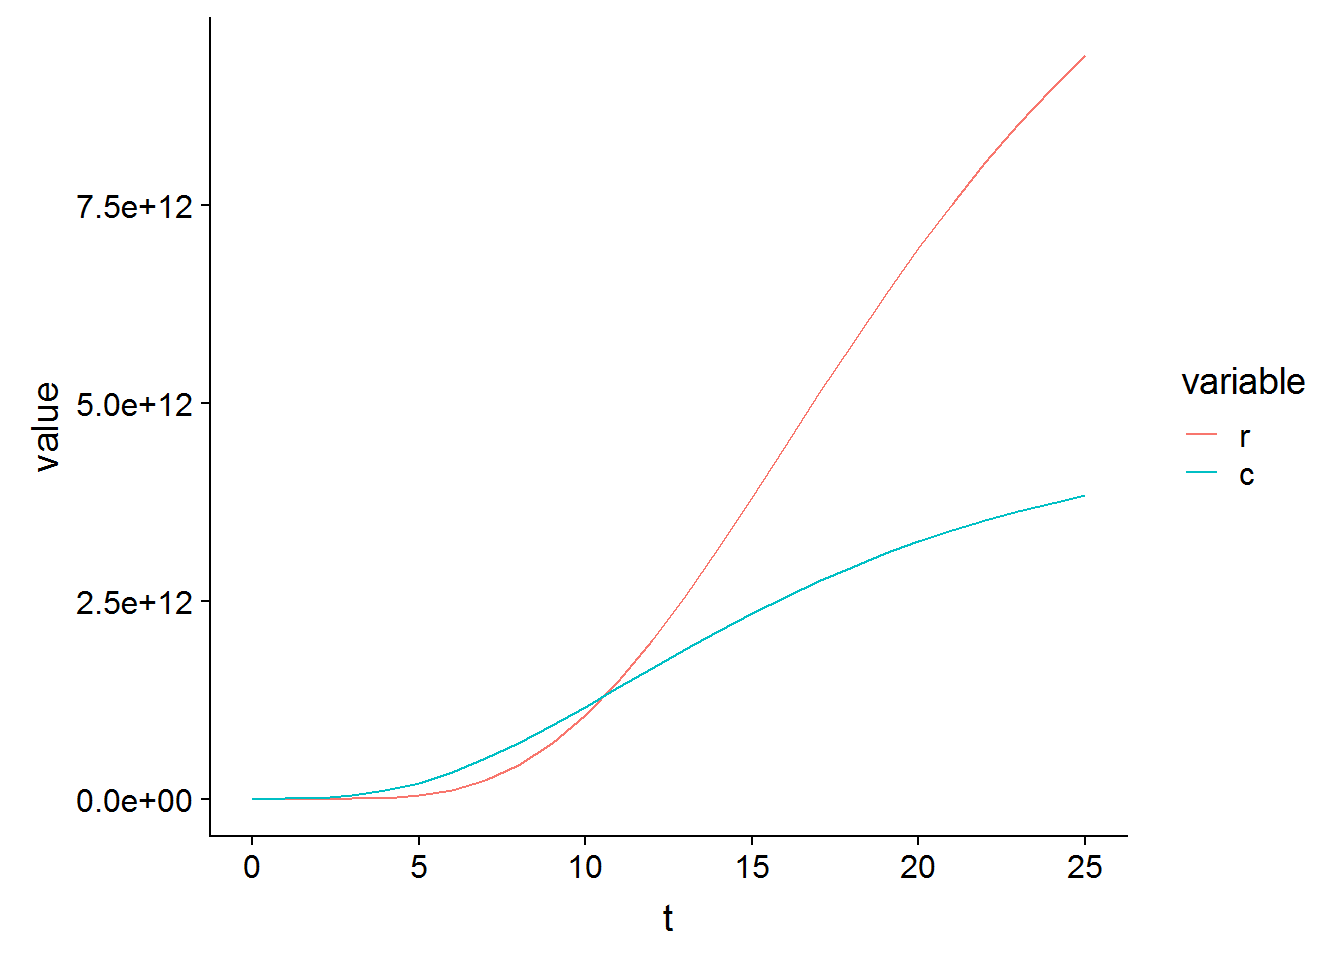
\includegraphics{aquaculture_files/figure-latex/demo_noharvest-1.pdf}

\subparagraph{Single Run, Harvest Demo}\label{single-run-harvest-demo}


\end{document}
